\pdfminorversion=7
\documentclass[usepdftitle=false, svgnames, color="table, fixpdftex, hyperref, fixinclude, xcdraw", t]{beamer}

\usepackage{lode-i18n}
\usepackage{lode-srccode}
\usepackage{lode-imacid}
\usepackage{lode-pdf}

\usepackage{animate}
\usepackage{movie15}

\title{Software testing}
\subtitle{JUnit}
\author[]{%
Marco Aur�lio Graciotto Silva\inst{1}, \and
Ellen Francine Barbosa\inst{1}, \\\and
Jos� Carlos Maldonado\inst{1}}

\newcommand{\numberofinstitutes}{2}
\institute[ICMC]
{
	\inst{1}%
%	\textbf{Institute of Mathematical Sciences and Computing}\\
	University of S�o Paulo (USP)\\
	S�o Carlos, SP, Brazil
	\and
	\inst{2}%
%	\textbf{Institute of Informatics}\\
	Federal University of Goi�s (UFG)\\
	Goi�nia, GO, Brazil
}

\date[]{February 2011}

\logopicture{resources/Logo/icmc-qualipso-inf}

\begin{document}

\frontmatter{}
../CommonAssets/preamble.tex



\mainmatter{}
\part{JUnit}
\section{JUnit}
\begin{frame}[c, parent={cmap:software-testing}, hasprev=false, hasnext=false]
\frametitle{JUnit}
\label{cmap:junit}

\insertcmap{Courses-SoftwareTesting-JUnit}
\end{frame}


\begin{frame}[parent={cmap:junit}, hasprev=false, hasnext=true]
\frametitle{JUnit}
\label{concept:junit}

\begin{block:concept}{What is it?}
JUnit is an open-source framework to provide support for documenting and
automating the execution of test sets for Java programs.
\end{block:concept}


\begin{block:fact}{General information}
\begin{itemize}
	\item Developed by Kent Beck and Erich Gamma (in 1994).

	\item Hosted at \url{http://www.junit.org/} and
	\url{http://sf.net/projects/junit/}.
\end{itemize}
\end{block:fact}


\begin{block:fact}{Features}
\begin{itemize}
	\item Test cases implemented using annotations.

	\item Useful assertions collection.

	\item Fixtures enhances the design of test sets.
\end{itemize}
\end{block:fact}

\hfill
\refie{example:identifier-testcases-junit}{\beamerbutton{Example: Identifier}}
\end{frame}



\begin{frame}[hasprev=true, hasnext=true]
\frametitle{JUnit}
\framesubtitle{Installation}
\label{procedure:junit:installation}


\begin{block:fact}{Requirements}
\begin{itemize}
	\item JUnit requires the Java Development Kit version 1.5 or newer.
\end{itemize}
\end{block:fact}

\begin{block:procedure}{Download}
\begin{enumerate}
	\item Download JUnit at \url{http://sourceforge.net/projects/junit/}.
	\begin{itemize}
		\item Current version is 4.8.1.

		\item The application is distributed as a JAR file (comprised of just
		the JUnit library) and a compressed ZIP file (with the JUnit library
		and documentation).

		\item Download the ZIP file.
	\end{itemize}

	\item Uncompress the file on a given directory that you have written
	permission.
\end{enumerate}
\end{block:procedure}
\end{frame}


\begin{frame}[fragile]
\frametitle{JUnit}
\framesubtitle{Configuration}
\label{procedure:junit:configuration}

\begin{block:fact}{How to run it?}
\begin{itemize}
	\item To execute the JUnit application, you must add the JUnit library
	(junit-4.8.1.jar) to the Java Classpath.
\end{itemize}
\end{block:fact}

\begin{block:fact}{Classpath configuration}
\begin{itemize}
	\item You can add the library to the CLASSPATH environment variable.
\begin{lstlisting}
Unix: \srccode{export CLASSPATH=/opt/junit-4.8.1/junit-4.8.1.jar:$CLASSPATH}
Windows: \srccode{set CLASSPATH=C:\junit-4.8.1\junit-4.8.1.jar;%CLASSPATH%}
\end{lstlisting}

	\item You can use the -cp option when running the tests. This is the
	recommended option!
\begin{lstlisting}
java -cp /opt/junit-4.8.1/junit-4.8.1.jar <program>
\end{lstlisting}
\end{itemize}
\end{block:fact}
\end{frame}



\begin{frame}[hasprev=true, hasnext=false]
\frametitle{JUnit}
\framesubtitle{Shake down}
\label{procedure:junit:shakedown}


\begin{block:fact}{Is it working?}
\begin{itemize}
	\item To check whether JUnit was correctly installed, you can run the JUnit
	test suite.
	\begin{itemize}
		\item The class with all the test cases for JUnit is
		\srccode{org.junit.tests.AllTests}.

		\item This class is located at the root of JUnit installation directory.
	\end{itemize}
\end{itemize}
\end{block:fact}


\hfill
\refie{example:junit-shakedown}{\beamerbutton{Example: JUnit shakedown}}
\end{frame}




\subsection{Test case}
\begin{frame}[parent={cmap:jabuti-gui},hasnext=true,hasprev=true]
\frametitle{Main functionalities}
\framesubtitle{Test Case Menu}
\label{concept:test-case-menu}

\begin{block}{Test case}
The \highlight{Test Case} menu provides options for test set manipulation and
report generation.
\end{block}

\begin{block}{Demo}
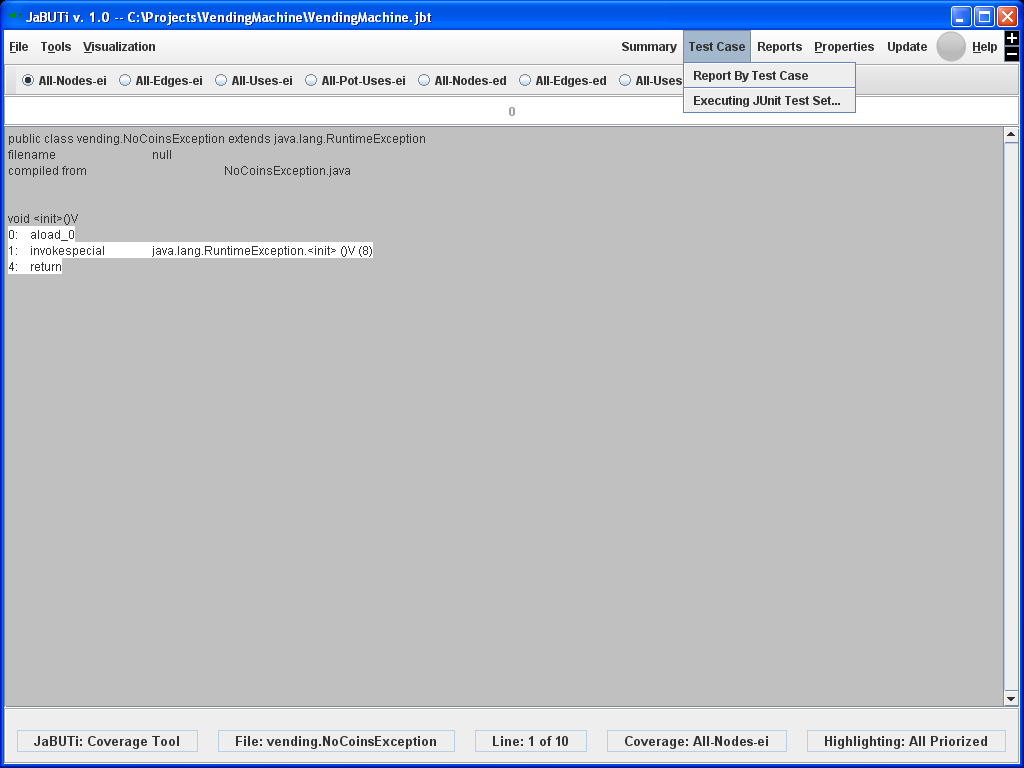
\includegraphics[width=\textwidth,clip]{resources/JaBUTi/JaBUTi-GUI/JaBUTi-GUI-TestCase/JaBUTi-GUI-TestCase}
\end{block}
\end{frame}



\begin{frame}
\frametitle{Main functionalities}
\framesubtitle{Test Case Menu}
\label{concept:report-by-test-case}

\begin{block}{Report By Test Case}
\highlight{Report By Test Case} option shows the coverage information with
respect to the current selected test criterion, for each individual test case,
considering all class under testing, and also allows to enable/disable and
delete/undelete test cases.
\end{block}

\begin{block}{Demo}
\insertmovie{JaBUTi/JaBUTi-GUI/JaBUTi-GUI-TestCase-ReportByTestCase/JaBUTi-GUI-TestCase-ReportByTestCase}
\end{block}
\end{frame}



\begin{frame}
\frametitle{Main functionalities}
\framesubtitle{Test Case Menu}
\label{concept:importing-from-junit}

\begin{block}{Importing from JUnit}
\highlight{Importing from JUnit} option allows to import a test set generated
according to the JUnit framework.
\end{block}

\begin{block}{Demo}
\insertmovie{JaBUTi/JaBUTi-GUI/JaBUTi-GUI-TestCase-ExecutingJUnitTestSet/JaBUTi-GUI-TestCase-ExecutingJUnitTestSet}
\end{block}
\end{frame}



\subsection{Test suite}
\begin{frame}[parent={concept:junit}, hasprev=false, hasnext=false]
\frametitle{JUnit test suite and suite runner}
\label{concept:junit-test-suite}
\label{concept:test-suite}

\begin{block:concept}{Test suite}
A JUnit test suite is a class that contains tests from many JUnit test
cases classes.
\end{block:concept}

\begin{block:procedure}{How to define a test suite?}
\begin{itemize}
	\item To create a JUnit test suite, the class (which is usually empty)
	should be annotated with \srccode{@SuiteClasses({TestClass1.class, ...})}.

	\item To run the JUnit test suite, the class must be annotated with
	\srccode{@RunWith(Suite.class)}
\end{itemize}
\end{block:procedure}

\hfill
\refie{example:junit-test-suite}{\beamerbutton{Example: JUnit test suite}}
\end{frame}


\subsection{Assertion}
\begin{frame}[parent={concept:junit}, hasprev=false, hasnext=true]
\frametitle{Assertion}
\label{concept:assertion}
\label{concept:junit-assertion}

\begin{block:concept}{Assertion}
An assertion is a statement that evaluates as true.
\end{block:concept}

\begin{block:fact}{}
\begin{itemize}
	\item Assertions work as oracles: they confront obtained and expected
	outputs, pointing any discrepancies, and enabling the automatic test
	cases execution.

	\item JUnit only records failed assertions.
\end{itemize}
\end{block:fact}

\hfill
\refie{example:junit-raw-assertion}{\beamerbutton{Example: Test case with assertion}}
\end{frame}


\begin{frame}[hasprev=true, hasnext=false]
\frametitle{Assertion}
\framesubtitle{JUnit assertions}

\begin{block:fact}{JUnit assertions}
\begin{itemize}
	\item Instead of using Java's default assertion mechanism, one can use
	assertions provided by JUnit.

	\item JUnit implements several assertions in the class \srccode{Assert}:
	\begin{itemize}
		\item \srccode{assertThat}
		\item \srccode{assertArrayEquals}, \srccode{assertEquals}
		\item \srccode{assertSame}, \srccode{assertNotSame}
		\item \srccode{assertTrue}, \srccode{assertFalse}
		\item \srccode{assertNull}, \srccode{assertNotNull}
		\item \srccode{fail}
	\end{itemize}
\end{itemize}
\end{block:fact}
\end{frame}

\subsubsection{Identity assertion}
\begin{frame}[parent={concept:assertion}, hasprev=false, hasnext=false]
\frametitle{Assertion}
\framesubtitle{Identity assertion}
\label{concept:junit-identity-assertion}
\label{concept:identity-assertion}

\begin{block:concept}{Identity assertion}
Identity assertions checks if two objects refer to the same object or not.
\end{block:concept}

\begin{block:fact}{Methods}
\begin{itemize}
	\item assertSame
	\item assertNotSame
\end{itemize}
\end{block:fact}

\hfill
\refie{example:junit-identity-assertion}{\beamerbutton{Example: Identity assertion}}
\end{frame}

\subsubsection{Nullity assertion}
\begin{frame}[parent={concept:assertion}, hasprev=false, hasnext=false]
\frametitle{Assertion}
\framesubtitle{Nullity assertion}
\label{concept:junit-nullity-assertion}
\label{concept:nullity-assertion}

\begin{block:concept}{Nullity assertion}
Nullity assertions check if an object is null.
\end{block:concept}

\begin{block:fact}{Methods}
\begin{itemize}
	\item \srccode{assertNull}
	\item \srccode{assertNotNull}
\end{itemize}
\end{block:fact}

\hfill
\refie{example:junit-nullity-assertion}{\beamerbutton{Example: Nullity assertion}}
\end{frame}

\subsubsection{Equality assertion}
\begin{frame}[parent={concept:assertion}, hasprev=false, hasnext=false]
\frametitle{Assertion}
\framesubtitle{Equality assertion}
\label{concept:junit-equality-assertion}
\label{concept:equality-assertion}

\begin{block:concept}{Equality assertion}
Equality assertions checks if the objects are equal (has the same content).
\end{block:concept}

\begin{block:fact}{Equality and identity}
\begin{itemize}
	\item Identity assertion implies Equality assertion.
\end{itemize}
\end{block:fact}

\begin{block:fact}{Methods}
\begin{itemize}
	\item \srccode{assertArrayEquals}
	\item \srccode{assertEquals}
\end{itemize}
\end{block:fact}

\hfill
\refie{example:junit-equality-assertion}{\beamerbutton{Example: Equality assertion}}
\end{frame}

\subsubsection{Exception assertion}
\begin{frame}[parent={concept:assertion}, hasprev=false, hasnext=false]
\frametitle{Assertion}
\framesubtitle{Exception assertion}
\label{concept:junit-exception-assertion}
\label{concept:exception-assertion}

\begin{block:concept}{Exception assertion}
An Exception assertion checks whether an exception is thrown by the test case.
\end{block:concept}


\begin{block:fact}{Annotation}
\begin{itemize}
	\item If the JUnit test case expects an exception to be thrown, it must
	declare the expected exception in the @Test annotation, at the
	\srccode{expected} parameter
	\begin{itemize}
		\item (e.g., \srccode{@Test(expected=IndexOutOfBoundsException.class)}.
	\end{itemize}
\end{itemize}
\end{block:fact}

\hfill
\refie{example:junit-exception-assertion}{\beamerbutton{Example: Exception assertion}}
\end{frame}

\subsubsection{Timing assertion}
\begin{frame}[parent={concept:assertion}, hasprev=false, hasnext=false]
\frametitle{Assertion}
\framesubtitle{Timing assertion}
\label{concept:junit-timing-assertion}
\label{concept:timing-assertion}

\begin{block:concept}{Timing assertion}
A timing assertion checks if the test case is executed in a given time frame.
\end{block:concept}


\begin{block:fact}{Annotation}
\begin{itemize}
	\item JUnit test cases can be annotated with a \srccode{timeout} parameter
	\begin{itemize}
		\item E.g., \srccode{@Test(timeout=2000)}
	\end{itemize}

	\item If the test takes longer than the specified number of milliseconds to
	run, the test fails.
\end{itemize}
\end{block:fact}

\hfill
\refie{example:junit-timing-assertion}{\beamerbutton{Example: Timing assertion}}
\end{frame}

\subsubsection{Truth assertion}
\begin{frame}[parent={concept:assertion}, hasprev=false, hasnext=false]
\frametitle{Assertion}
\framesubtitle{Truth assertion}
\label{concept:junit-truth-assertion}
\label{concept:truth-assertion}

\begin{block:concept}{Truch assertion}
A truth assertion checks if a condition is true or false.
\end{block:concept}


\begin{block:fact}{Methods}
\begin{itemize}
	\item assertTrue
	\item assertFalse
\end{itemize}
\end{block:fact}

\hfill
\refie{example:junit-truth-assertion}{\beamerbutton{Example: Truth assertion}}
\end{frame}

\subsubsection{Condition matching assertion}
\begin{frame}[parent={concept:assertion}, hasprev=false, hasnext=false]
\frametitle{Assertion}
\framesubtitle{Condition matching assertion}
\label{concept:junit-condition-matching-assertion}
\label{concept:condition-matching-assertion}

\begin{block:concept}{Condition matching assertion}
A condition matching assertion checks whether a given object matches the
condition specified by the assertion.
\end{block:concept}

\begin{block:fact}{Method}
\begin{itemize}
	\item \srccode{assertThat}
	\begin{itemize}
		\item The AssertThat assertion provides more readable and typeable
		statements, combinations of any matcher statement, more readable
		failure messages, and custom matchers.
	\end{itemize}
\end{itemize}
\end{block:fact}

\hfill
\refie{example:junit-condition-matching-assertion}{\beamerbutton{Example: Condition matching assertion}}
\end{frame}


\subsection{Fixture}
\begin{frame}[parent={concept:junit}, hasprev=false, hasnext=false]
\frametitle{Fixture}
\label{concept:junit-fixture}
\label{concept:fixture}

\begin{block:concept}{Fixture}
\begin{itemize}
	\item Fixtures are actions that should be executed before or after a test
	case (usually to set up pre-conditions).

	\item It defines a fixed state of a set of objects used as a baseline for
	running tests.
\end{itemize}
\end{block:concept}

\begin{block:fact}{Why should I use fixtures?}
\begin{itemize}
	\item The purpose of a test fixture is to ensure that there is a well known
	and fixed environment in which tests are run so that results are
	repeatable.
\end{itemize}
\end{block:fact}
\end{frame}

\subsubsection{Before}
\begin{frame}[parent={concept:fixture}, hasprev=false, hasnext=false]
\frametitle{Fixture}
\framesubtitle{Before}
\label{concept:junit-before-fixture}
\label{concept:before-fixture}
\label{concept:before}

\begin{block:concept}{Before fixture}
Before is a fixture that is used to set up pre-conditions for a test
case.
\end{block:concept}

\begin{block:fact}{How to use it?}
\begin{itemize}
	\item The Before fixture is created by annotating a method with
	\srccode{@Before}.

	\item Before fixtures run before a JUnit test case.

	\item Before fixtures declared in the superclasses will be run before those
	of the current class.

	\item No ordering is defined when running Before fixtures declared in the
	same class.
\end{itemize}
\end{block:fact}
\end{frame}

\subsubsection{BeforeClass}
\begin{frame}[parent={concept:fixture}, hasprev=false, hasnext=false]
\frametitle{Fixture}
\framesubtitle{BeforeClass}
\label{concept:junit-beforeclass-fixture}
\label{concept:beforeclass-fixture}
\label{concept:beforeclass}

\begin{block:concept}{BeforeClass}
BeforeClass is a fixture that is used to set up preconditions for a
test set.
\end{block:concept}


\begin{block:fact}{How to use it?}
\begin{itemize}
	\item The BeforeClass fixture is created by annotating a method with
	\srccode{@BeforeClass}.

	\item BeforeClass fixtures run before all the JUnit test cases in a class
	have been run.

	\item BeforeClass fixtures declared in the superclasses will be run after
	those of the current class.

	\item No other ordering is defined when running BeforeClass fixtures
	declared in the same class.
\end{itemize}
\end{block:fact}
\end{frame}

\subsubsection{After}
\begin{frame}[parent={concept:fixture}, hasprev=false, hasnext=false]
\frametitle{Fixture}
\framesubtitle{After}
\label{concept:junit-after-fixture}
\label{concept:after-fixture}
\label{concept:after}

\begin{block:concept}{After}
After is a fixture that is used to cleanup modifications made for or
by a test case.
\end{block:concept}

\begin{block:fact}{How to use it?}
\begin{itemize}
	\item The After fixture is created by annotating a method with
	\srccode{@After}.

	\item After fixtures run after a JUnit test case.

	\item After fixtures declared in the superclasses will be run before those
	of the current class.

	\item No ordering is defined when running After fixtures declared in the
	same class.
\end{itemize}
\end{block:fact}
\end{frame}

\subsubsection{AfterClass}
\begin{frame}[parent={concept:fixture}, hasprev=false, hasnext=false]
\frametitle{Fixture}
\framesubtitle{AfterClass}
\label{concept:junit-afterclass-fixture}
\label{concept:afterclass-fixture}
\label{concept:afterclass}

\begin{block:concept}{AfterClass}
AfterClass is a fixture that is used to cleanup modifications made
for or by a test set.
\end{block:concept}


\begin{block:fact}{How to use it?}
\begin{itemize}
	\item The AfterClass fixture is created by annotating a method with
	\srccode{@AfterClass}.

	\item AfterClass fixtures run after all the JUnit test cases in a class
	have been run.

	\item AfterClass fixtures declared in the superclasses will be run after
	those of the current class.

	\item No other ordering is defined when running AfterClass fixtures
	declared in the same class.
\end{itemize}
\end{block:fact}
\end{frame}



\backmatter{}
\part{References and credits}
\part{References}
\section*{References}


\begin{frame}[label=references, allowframebreaks]{\refname}
\bibliographystyle{abnt-num}
\bibliography{root}
\end{frame}

\part{Acknowledgement}
\section*{Acknowledgement}


\begin{frame}[c,label=credits]
\frametitle{Credits}

\begin{itemize}
	\item Reviewers:
	\begin{itemize}
		\item Marcio Eduardo Delamaro
	\end{itemize}
\end{itemize}
\end{frame}


\part{Instructional elements}
\section{Examples}


% Structural software testing
%
\part{Structural software testing}
\subsection{Control flow graph}
\insertexample{identifier-cfg}{concept:cfg-graph-elements}

\subsection{Definition-use graph}
\insertexample{program-graph}{concept:definition-use-graph}

\subsection{Identifier definition-use graph}
\insertexample{identifier-dug}{concept:definition-use-graph}


% Path
%
\part{Path}
\subsection{Infeasible path}
\insertexample{identifier-infeasible-path}{concept:infeasible-path}

\subsection{Complete path}
\insertexample{identifier-complete-path}{concept:complete-path}

\subsection{Definition-clear paths example}
\insertexample{identifier-def-clear-path}{concept:definition-clear-path}


% Control flow test criterion
%
\part{Control-flow based testing}
\subsection{All-nodes}
\insertexample{all-nodes}{concept:all-nodes}

\subsection{All-paths infeasibility}
\insertexample{all-paths}{concept:all-paths}


% Complexity-based test criterion
%
\part{Complexity-flow based testing}
\subsection{McCabe example}
\insertexample{mccabe}{procedure:mccabe-criterion}


% Data flow test criterion
%
\part{Data-flow based testing}
\subsection{All-Uses for Identifier}
\insertexample{identifier-all-uses}{concept:all-uses}

\subsection{All-Pot-Uses for Identifier}
\insertexample{identifier-all-pot-uses}{concept:all-pot-uses}

\section{Exercises}



\end{document}
